\documentclass[12pt,a4paper,titlepage]{article}

\usepackage{graphicx}
\usepackage{indentfirst}
\usepackage[usenames,dvipsnames]{color}
\usepackage{fancyvrb} % for verbatim
\usepackage{fancyhdr}
\usepackage{listings}
\usepackage[sf]{titlesec}
\usepackage{titletoc}
\usepackage[boldfont,slantfont,CJKnumber]{xeCJK}
\usepackage{xcolor} % 使用颜色宏包

\definecolor{steelblue}{rgb}{.275,.51,.71}
\definecolor{lpink}{rgb}{.991,.711,.754}
\definecolor{mygray}{gray}{0.92}
\definecolor{darkblue}{rgb}{0,0,.5}
\definecolor{darkgreen}{rgb}{0,.39,0}
\definecolor{hgray}{gray}{.5}
\definecolor{lgray}{gray}{.8}

\usepackage[colorlinks=true,urlcolor=blue,linkcolor=blue]{hyperref} % for links and anchors

\setCJKmainfont[BoldFont=Adobe Heiti Std]{Adobe Song Std} % 设置默认的中文字体
\setCJKfamilyfont{kai}{Adobe Kaiti Std}

\newcommand{\kai}{\CJKfamily{kai}}
\newcommand{\sectionname}{第\CJKnumber{\thesection}章}
\newcommand{\myheader}[1]{\textcolor{darkblue}{#1}}

\renewcommand\contentsname{目录}

\newcommand\refsite{\section{附录}
您可以在\href{http://i-math.appspot.com/}{\color{blue}http://i-math.appspot.com/}访问该站点。}
\special{ pdf: bgcolor [ 1.00 0.98 0.95 ] }

 \linespread{1.36}

\pagestyle{fancy}

\rhead{\textcolor{hgray}{JerryMouse}}
\fancyhead[LE,LO]{\textcolor{hgray}\leftmark} 

\makeatletter
\renewcommand{\maketitle}{\begin{titlepage}%
\let\footnotesize\small
    \let\footnoterule\relax
    \parindent \z@
    \reset@font
    \vskip 10\p@
    \hbox{\mbox{%
        \hspace{4pt}%
        
\includegraphics[width=6em]{data/logo.jpeg}
        \hspace{4pt}
        }%
     \vrule depth 0.8\textheight%
      \mbox{\hspace{2em}}
      \vtop{% %%%%%%%%%%%%%%%%%%
        \vskip 40\p@
        \begin{flushleft}
          \Large \@author \par
        \end{flushleft}
        \vskip 80\p@
        \begin{flushleft}
        \textcolor{steelblue}{ \fontsize{36}{20pt} \bfseries \kai \@title }\par
        \end{flushleft}
        \vfil
        }}

  \end{titlepage}%
}

\makeatother


\titleformat{\section}[hang]{\LARGE\sf\kai}
            {\myheader\sectionname}
            {1em}
            {\myheader}[\color{steelblue}{\titlerule}]

\titleformat{\subsection}[hang]{\Large\sf\kai}
            {\myheader\thesubsection}
            {1em}
            {\myheader}
\titleformat{\subsubsection}[hang]{\large\sf\kai}
            {\myheader\thesubsubsection}
            {1em}
            {\myheader}


\titlecontents{section}
              [2em]{\large\sf\kai\addvspace{-0.1em}}
              {\thecontentslabel\quad}
%%            {\hspace*{-2.3em}}
              {}
              {\titlerule*[0.8pc]{.}\contentspage}
\titlecontents{subsection}
              [4em]{\small\addvspace{-0.2em}}
              {\thecontentslabel\quad}
%%            {\hspace*{-2.3em}}
              {}
              {\titlerule*[0.8pc]{.}\contentspage}
\titlecontents{subsubsection}
              [6em]{\small\addvspace{-0.2em}}
              {\thecontentslabel\quad}
%%            {\hspace*{-2.3em}}
              {}
              {\titlerule*[0.8pc]{.}\contentspage}



\lstset{
keywordstyle=\color{blue!70}, commentstyle=\color{red!50!green!50!blue!50},
frame=shadowbox,
rulesepcolor=\color{red!20!green!20!blue!20}
}
\lstset{breaklines}%这条命令可以让LaTeX自动将长的代码行换行排版
\lstset{extendedchars=false}

% \lstset{ xleftmargin=2em,xrightmargin=2em, aboveskip=1em}

\title{iMath作品说明}
\author{Jerry Mouse}
\date{\today}

\graphicspath{{data/}} %%图片路径

\begin{document}

\maketitle

\tableofcontents

\clearpage

\section{引言}

\subsection{编写目的}
\paragraph{}
 为了方便大家快速融入iMath, 特编写此说明书。
\paragraph{}
 此说明书供有意尝试、使用iMath的同学们参考。

\subsection{说明}
\begin{itemize}
\item 项目名称:iMath
\item 团队名称:JerryMouse
\item 团队所属机构:南京大学
\item 开发项目组信息:
\begin{center}
\begin{tabular}{|l|l|l|l|}
\hline
\begin{tabular}[t]{l}角色\end{tabular} &
\begin{tabular}[t]{l}学号\end{tabular} &
\begin{tabular}[t]{l}姓名\end{tabular} &
\begin{tabular}[t]{l}电子邮件\end{tabular}\\
\hline
\begin{tabular}[t]{l}PM\end{tabular} &
\begin{tabular}[t]{l}071251184\end{tabular} &
\begin{tabular}[t]{l}颜开\end{tabular} &
\begin{tabular}[t]{l}kaiyannju@gmail.com\end{tabular}\\
\hline
\begin{tabular}[t]{l}TM\end{tabular} &
\begin{tabular}[t]{l}071251175\end{tabular} &
\begin{tabular}[t]{l}徐建国\end{tabular} &
\begin{tabular}[t]{l}pkpb@sohu.com\end{tabular}\\
\hline
\begin{tabular}[t]{l}TM\end{tabular} &
\begin{tabular}[t]{l}071251173\end{tabular} &
\begin{tabular}[t]{l}徐博翰\end{tabular} &
\begin{tabular}[t]{l}xbh07@software.nju.edu.cn\end{tabular}\\
\hline
\end{tabular}
\end{center}
\item 联系电话:15850736725 13585193542

\item 运行环境:标准浏览器
\item 开发环境 :  Linux,Maven,Ant,GAE
\end{itemize}

\section{概述}
\subsection{系统简介}
\paragraph{}
iMath是一个\textbf{开放}的\textbf{数学}网络\textbf{平台},提供各种数学服务和资源。
包括高等数学和统计运算,更重要的是他的开发式平台能够吸引各种人来制作分享自己的数学工具。(为了方便表述和架构原因,本文中的数学工具将被成为Gadget)

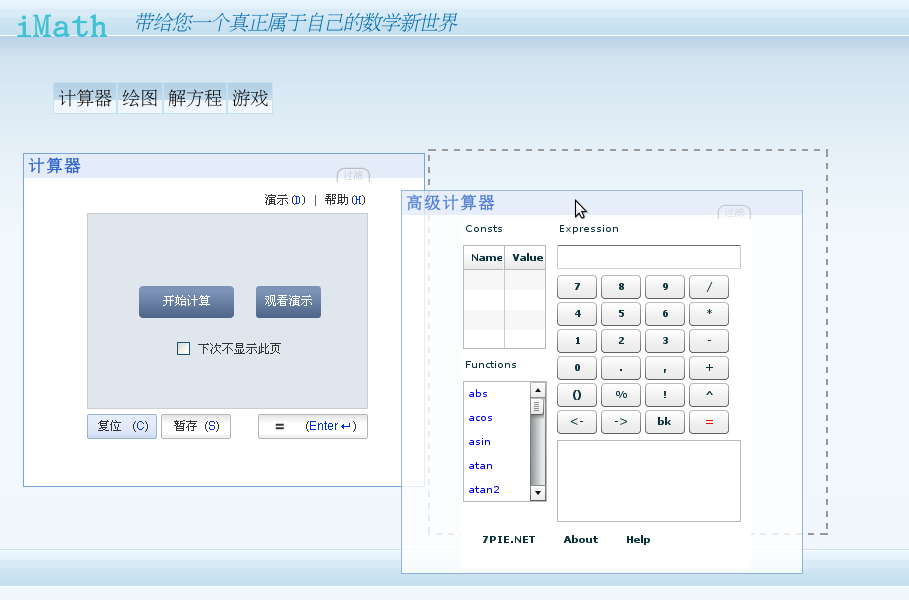
\includegraphics[width=\textwidth]{first.png}

\subsection{特色}

\subsubsection{开放式平台}
\paragraph{}
该平台几乎完全实现了Google  Gadgets API,并扩展之,使Gadgets之间有互操作的能力。这样,任何一个标准Gadget都可以部署在iMath上,使iMath成为一个真正的
开放平台。iMath中每一个数学工具都是一个Gadget。
\paragraph{}
以下是一个最简单的Gadget的代码
\begin{lstlisting}[language=xml]
<?xml version="1.0" encoding="UTF-8" ?> 
<Module>
  <ModulePrefs title="hello world example" /> 
  <Content type="html">
     <![CDATA[ 
       Hello, world!
     ]]>
  </Content> 
</Module>
\end{lstlisting}
您可以看到一个Gadget是非常简单的。您也可是试着为iMath编写一个Gadget。

\subsubsection{云计算}
\paragraph{}  
经过各大厂商长时间炒作,大家想必知道云计算\footnote{云计算(cloud computing,台湾译作云端运算),是一种动态的易扩展的且通常是通过互联网提供虚拟化的资源计算方式, 用户不需要了解云内部的细节,也不必具有云内部的专业知识,或直接控制基础设施。}。但很少有人见过真正的云。iMath便是构建在Google云计算平台上的云服务。
\paragraph{}
现在将由iMath来揭开云计算的神秘面纱。
在iMath的云端,运行的是集群服务器而不是普通的web容器,持久化使用的是BigTable而不是传统数据库。用户只可以通过一些接口来完成操作,
下图是从云端摘录的最近24小时运行情况:

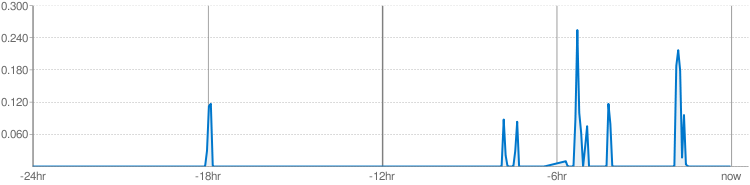
\includegraphics[width=\textwidth]{chart.png}

\subsubsection{web服务运算}
\paragraph{}
如果Gadget拥有者愿意,他可以开放他的服务接口。下图是一个利用Google Chart生成曲线图的接口。

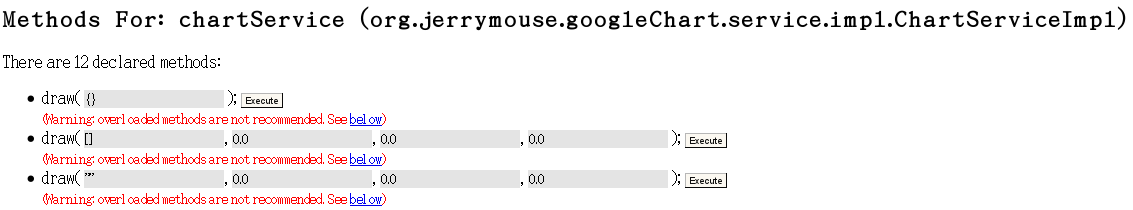
\includegraphics[width=\textwidth]{dwr.png}
\paragraph{}
其他软件提供商或者用户自身可以自由使用这些接口,而不用再关心背后的实现。
更重要的时,我们可以获得用户使用信息来\textbf{优化算法},以及\textbf{缓存结果}来大幅提高运行效率。

\section{功能}
\paragraph{}
以下是iMath的初期设计图,他体现了iMath的应有的功能。

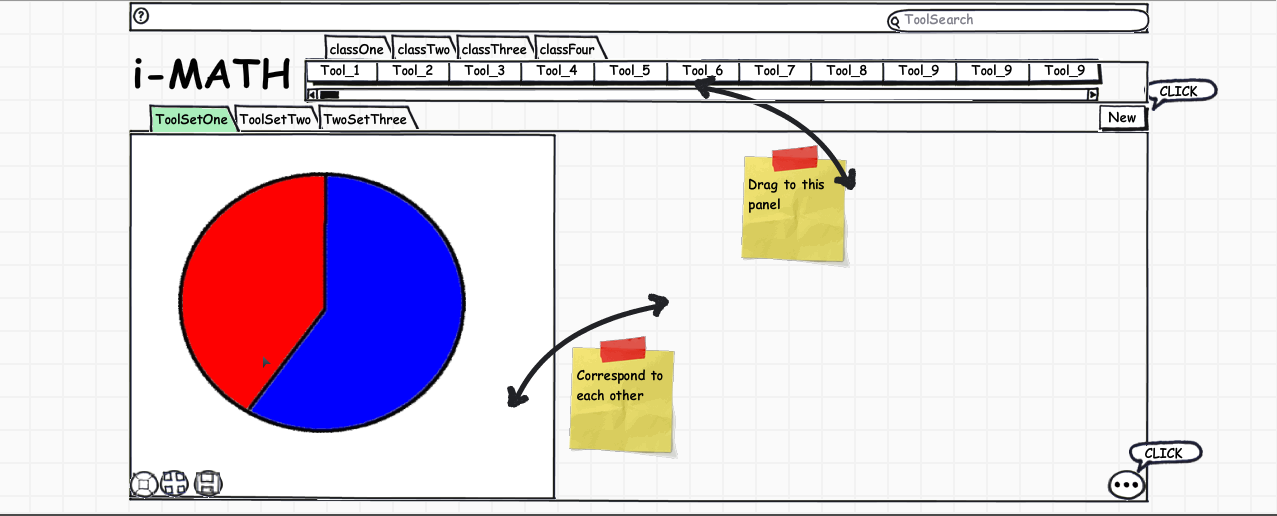
\includegraphics[width=\textwidth]{init1.1.png}

\paragraph{}
上方类似标签的是\textbf{工具集}。他可以是“绘图工具集合”也可以“方程工具集合”,您完全可以自由组合小工具来形成工具集,
比如您可以自制一个“绘图方程工具集合”,在解方程的同时进行绘图。

\paragraph{}
下方是小工具的\textbf{容器},您可以自由拖拽组合,当然也提供了搜索,添加甚至自定义小工具的功能。

\paragraph{}
目前含有的工具有:计算器,高级计算器,绘图器,解线性方程和数独 小游戏。
在开发的最后阶段,我们将大量生产更多的小工具。

\section{架构}

\subsection{目录结构及构建方式}

\subsubsection{源代码}
\paragraph{}
源代码地址:\href{http://code.google.com/p/i-math/}{\color{blue}http://code.google.com/p/i-math/}。
由于涉及到了云计算,构建极其复杂(可以写出长达100页的详细说明书),笔者并不试图让读者看过本文后能自己构建这个应用。

\subsubsection{目录结构}
\paragraph{}
以下是目录结构图:

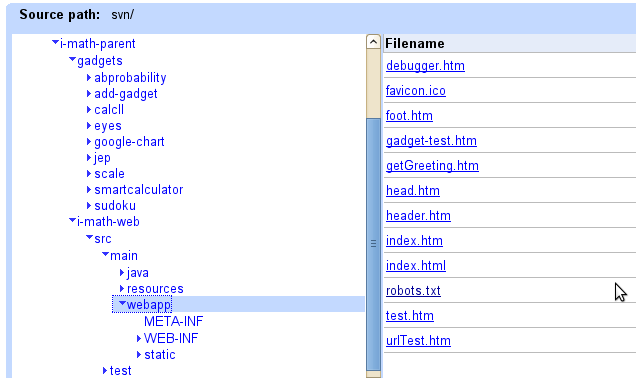
\includegraphics[width=\textwidth]{dic.png}

\paragraph{}
本项目i-math-parent使用gadgets和i-math-web两个子项目构成。i-math-web就是web平台,而gadgets是web工具。
通过maven复杂的构建\footnote{优化过的i-math-web的构建文件长达400行,而总共有近20个这样的构建文件},两者有机结合在了一个。
gadgets含有无数的子项目,他们每一个就是一个Gadget。

\subsubsection{i-math-web}
\paragraph{}

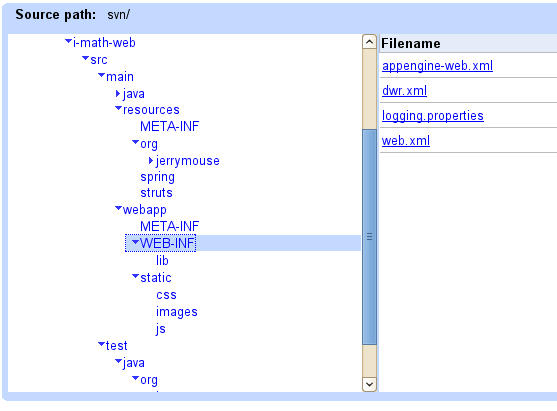
\includegraphics[width=\textwidth]{web.png}

\paragraph{}
i-math-web由gadget引擎,和gadget容器服务组成。gadget引擎负责解析符合Gadget API的xml文件和生成Gadget页面。而gadgett容器服务
则是支持用户来自定义自己的页面。具体内容过于复杂,不再赘述。

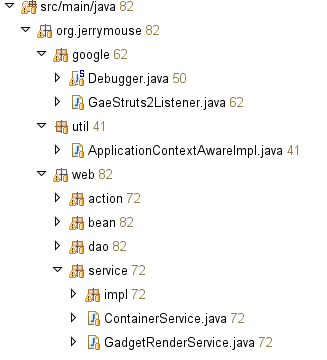
\includegraphics[width=\textwidth/2]{java.png}

\paragraph{}
\begin{itemize}
 \item 客户端技术:Mootools+Jquery+Dojo+$\cdots$。
\item 云端技术:Spring+Struts+Jdo+Appengine+Dwr+freemaker+$\cdots$。
\end{itemize}



\section{附录}
\paragraph{}
您可以在\href{http://i-math.appspot.com/}{\color{blue}http://i-math.appspot.com/}访问该站点。
由于使用云计算,服务器在美国,所以网速会比较慢,请耐心等待。相信在不远的将来,在中国的网速会得到提升。
另外为了方便您的浏览,请使用支持W3c标准的浏览器,推荐Chrome和Firefox。
\paragraph{}
此文成文时项目仍在开发阶段,故可能于最后成品不完全相符。
\end{document}
